\documentclass{beamer}

\usepackage[utf8]{inputenc} % Language and font encoding
\usepackage[icelandic]{babel}
\usepackage[T1]{fontenc}


\usepackage{tikz}
\usepackage[listings,theorems]{tcolorbox}
\usepackage{booktabs}
\usepackage{minted} %Minted and configuration
\usemintedstyle{default}

\renewcommand{\theFancyVerbLine}{\sffamily \arabic{FancyVerbLine}}
%%%%%%%%%%%
% More math
%%%%%%%%%%%
\newcommand{\Mod}[1]{\ \text{mod}\ #1}

%%%%%%%%%%%%%%%%%%%%%%
% Beamer configuration
%%%%%%%%%%%%%%%%%%%%%%
\setbeamertemplate{navigation symbols}{}
\usecolortheme{dove}
\setbeamercolor{frametitle}{fg=white}

\usebackgroundtemplate%
{%
\vbox to \paperheight{

\includegraphics[width=\paperwidth]{Pics/hi-slide-head-2016}

\vfill
\hspace{0.5cm}
\includegraphics[width=0.3\paperwidth]{Pics/hi-von-logo}
\vspace{0.4cm}
    }%
}

\AtBeginSection[]
{
  \begin{frame}<beamer>
    \frametitle{Yfirlit}
    \tableofcontents[currentsection]
  \end{frame}
}

\setbeamerfont{frametitle}{size=\normalsize}
\addtobeamertemplate{frametitle}{}{\vspace*{0.5cm}}

%%%%%%%%%%%%%%%%%%%%%%%%%
% tcolorbox configuration
%%%%%%%%%%%%%%%%%%%%%%%%%

% Setup from: http://tex.stackexchange.com/a/43329/21638
\tcbset{%
    noparskip,
    colback=gray!10, %background color of the box
    colframe=gray!40, %color of frame and title background
    coltext=black, %color of body text
    coltitle=black, %color of title text 
    fonttitle=\bfseries,
    alerted/.style={coltitle=red, colframe=gray!40},
    example/.style={coltitle=black, colframe=green!20, colback=green!5},
}


%%%%%%%%%%%%%%%%%%%%%%%
% Further configuration
%%%%%%%%%%%%%%%%%%%%%%%
\hypersetup{colorlinks=true,pdfauthor={Eirikur Ernir Thorsteinsson},linkcolor=blue,urlcolor=blue}
\graphicspath{{./Pics/}}

\author{Eiríkur Ernir Þorsteinsson}
\institute{Háskóli Íslands}
\date{Haust 2016}

\title{Tölvunarfræði 1a}
\subtitle{Vika 4, fyrri fyrirlestur}

\begin{document}

\begin{frame}
\titlepage
\end{frame}

\section{Inngangur}


\begin{frame}{Í síðasta þætti\ldots}
\begin{itemize}
 \item Inntak og úttak
 \begin{itemize}
  \item \texttt{input}
  \item \texttt{fprintf}
 \end{itemize}
 \item Einfaldar myndir
 \begin{itemize}
  \item \texttt{plot}
 \end{itemize}
\end{itemize}
Kaflar: 3.3 til 3.6
\end{frame}

\begin{frame}{Um spurningu 5 í skiladæmunum}
\begin{center}
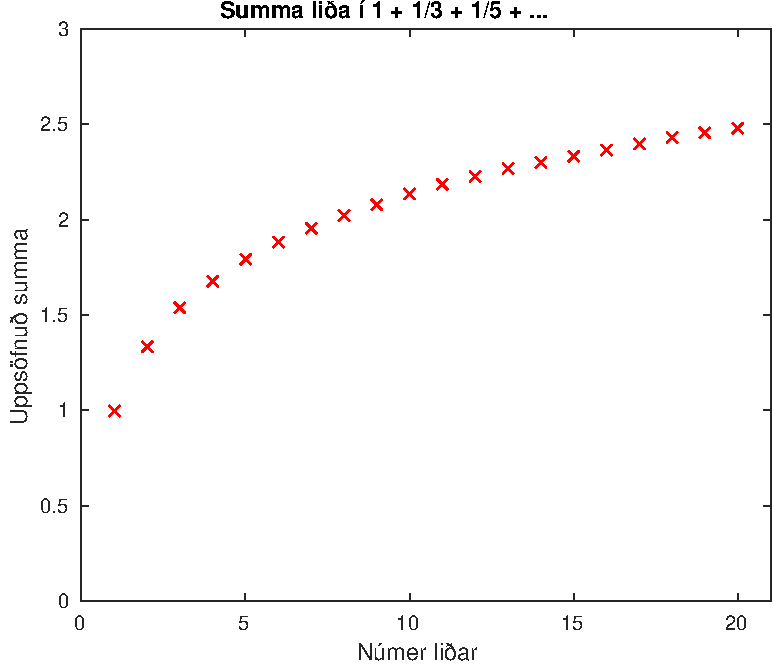
\includegraphics[width=0.8\textwidth]{sum-plot}
\end{center}

\end{frame}


\section{Inntak og úttak með skrám}

\begin{frame}{Einfalt inntak og útták með skrám}
\begin{itemize}
 \item Þegar unnið er með mikið gagnamagn er gott að geyma gögn í skrám
 \item Skipunin \texttt{save skráarnafn fylki -ascii} vistar gögnin í $fylki$ í skrá
 \begin{itemize}
  \item Ef skráin er þegar til er hún yfirskrifuð
  \item Skrifa má aftast í skrá í stað yfirskriftar með því að gefa valmöguleikann \texttt{-append}
 \end{itemize}
 \item Skipunin \texttt{load skráarnafn} les innihald skrár inní fylki
  \begin{itemize}
   \item Fylkið heitir sama nafni og skráin (án endingar)
  \end{itemize}
 \end{itemize}
\end{frame}

\begin{frame}[fragile]{Dæmi um skráarinntak og skráarúttak}
\begin{minted}[frame=lines]{matlab}
>> a = randi(5,2,2) % 2x2 slembifylki búið til
a =
   3   2
   3   4
>> save gogn.dat a -ascii % a skrifað í skrána gogn.dat
>> load gogn.dat % innihald gogn.dat sett í breytuna gogn
>> gogn
gogn =
   3   2
   3   4
\end{minted}
\end{frame}


\begin{frame}{Gömul fyrirlestraræfing}
\begin{columns}
\column{0.6\textwidth}
\begin{enumerate}
\setcounter{enumi}{2}
 \item Hér til hliðar eru hitamælingar fyrir septemberdag í Reykjavík. Sýnið snyrtilegt línurit fyrir hitastigið þennan dag.
 \item Vistið þessar upplýsingar í skrá.
\end{enumerate}
\column{0.4\textwidth}
\begin{center}
\begin{tabular}{ll}
\toprule
Klst&$C^\circ$\\
\midrule
0&12.5\\
3&12.4\\
6&12.3\\
9&12.8\\
12&13.4\\
15&14\\
18&13.1\\
21&12.8\\
\bottomrule
\end{tabular}
\end{center}
\end{columns}
\end{frame}

\begin{frame}[fragile]{Gömul fyrirlestrarræfing}
\begin{center}
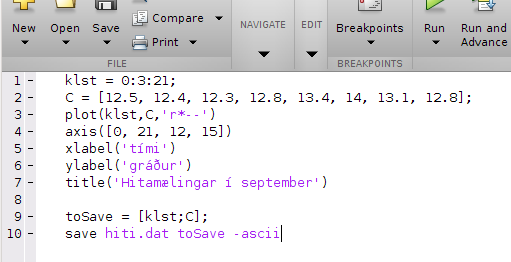
\includegraphics[width=0.9\textwidth]{Pics/septemberhitiscript}
\end{center}
\end{frame}

\begin{frame}[fragile]{Gömul fyrirlestrarræfing}
\begin{center}
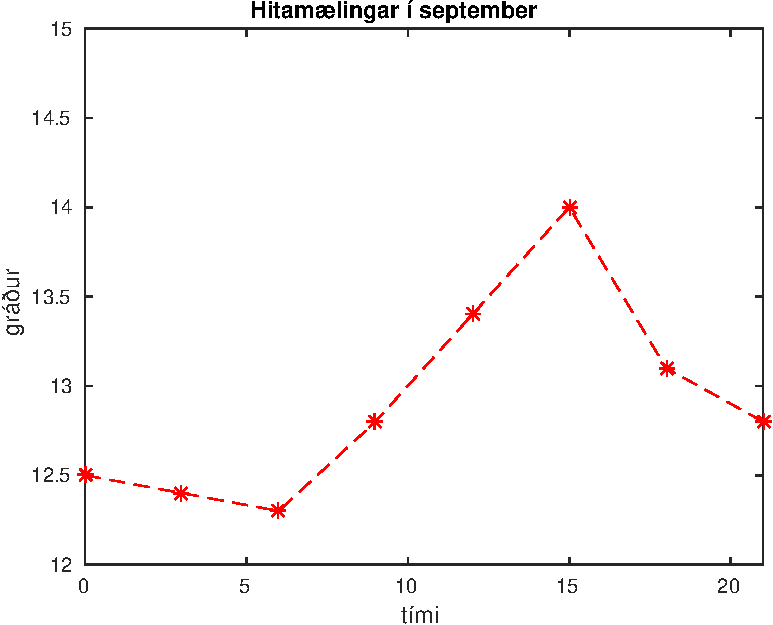
\includegraphics[width=0.7\textwidth]{Pics/septemberhiti}
\end{center}
\end{frame}

\section{Föll (3.7)}

\begin{frame}{Upprifjun á fallshugtakinu}
\begin{itemize}
 \item Föll eru notuð til að framkvæma ákveðna útreikninga sem \emph{byggja á inntaksgildum}
 \begin{itemize}
  \item Föllin taka inn gildi, reikna með gildunum, og skila niðurstöðu.
  \item Oftast er útkoman eitt gildi, niðurstaða útreikninga
 \end{itemize}
\end{itemize}
\end{frame}

\begin{frame}[fragile]{Hagnýt atriði}
\begin{itemize}
 \item Hafið hvert fall eitt og sér í skrá
 \begin{itemize}
  \item Nefnið skrána sama nafni og fallið, nema skráin hefur endinguna \texttt{.m}
 \end{itemize}
 \item Breyturnar og geta verið með jafn fjölskrúðug nöfn og aðrar breytur í Matlab
 \item Ekki nefna breytur og skipanaskrár sama heiti
\end{itemize}
\end{frame}

\begin{frame}[fragile]{Dæmi}
Dæmi: Fallið \texttt{distance}, sett í skrána \texttt{distance.m}.
\begin{minted}[frame=lines]{matlab}
function d = distance(v, t)
  d = v*t;
end  
\end{minted}
Þetta fall heitir \texttt{distance}, tekur inn breytu $v$ sem táknar (meðal)hraða, lengd tímabils $t$ og skilar fjarlægð. Eftir að það hefur verið skilgreint má nota það alls staðar í sömu Matlab-möppu (í skipanaglugga, í skipanaskrám, í öðrum föllum).
\end{frame}

\begin{frame}{Föll vs. skipanaskrár}
\begin{itemize}
 \item \emph{Mjög auðvelt} er að rugla saman hugtökunum um föll og skipanaskrár
 \begin{itemize}
  \item Hvort tveggja er geymt í skrá
 \end{itemize}
 \item Fall er safn af skipunum sem táknar ákveðna gerð af útreikningum
 \begin{itemize}
  \item Fyrsta orðið er \texttt{function}
  \item Inntök og úttök skilgreind í haus fallsins
 \end{itemize}
 \item Skipanaskrá er samansafn af hvaða Matlab-skipunum sem er
 \begin{itemize}
  \item Venjulega er inntak skilgreint með \texttt{input} og útskrift með \texttt{disp} eða \texttt{fprintf}
  \item Skipanaskrá \emph{skilar} ekki gildi!
 \end{itemize}
\end{itemize}
\end{frame}

\begin{frame}{Föll og skipanaskrár eru vinir}
Algengt mynstur:
\begin{itemize}
 \item Skipanaskrár lesa inntak og skrifa úttakið
 \item Föll framkvæma útreikninga
\end{itemize}

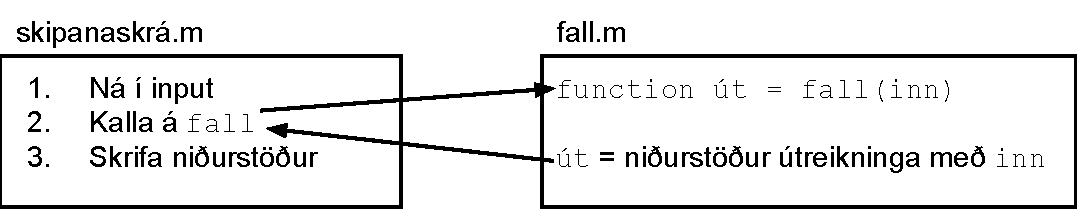
\includegraphics[width=\textwidth]{Pics/skripta-og-fall}
\end{frame}

\begin{frame}[fragile]{Forritunarvenjur}
\begin{columns}
\column{0.5\textwidth}
\begin{itemize}
 \item Algengt: Skjölun (e. \emph{documentation}), þ.e.a.s. staðlaðar athugasemdir efst í falli
 \begin{itemize}
  \item Lýsing á því hvað fallið gerir
  \item Hvernig á að kalla á fallið
  \item Form inntaksbreyta (stika)
  \item Form skilagildis
  \item Breytingasaga
 \end{itemize}
 \item Inndráttur
 \begin{itemize}
  \item Smart Indent (ctrl+i) í Matlab ritli gerir þetta fyrir okkur
 \end{itemize}
\end{itemize}
\column{0.5\textwidth}
\begin{minted}[frame=lines]{matlab}
function c = fahrToCelc(f)
% fahrToCelc breytir úr F í C
% Notkun:  fahrToCelc(fhiti)
   c = (f-32)*5/9;
end
\end{minted}

\end{columns}
\end{frame}

\subsection{Staðværar breytur}

\begin{frame}{Staðværar breytur}
\begin{itemize}
 \item Stundum þarf að skilgreina nýjar breytur inni í föllum
 \begin{itemize}
  \item Þær eru þá staðværar (e. \emph{local}) innan fallsins
  \item Þær hverfa úr minninu þegar fallið hefur lokið keyrslu
  \item Valda ekki árekstrum við aðrar breytur utan fallsins
 \end{itemize}
\end{itemize}
\end{frame}

\begin{frame}{Framkvæmd}
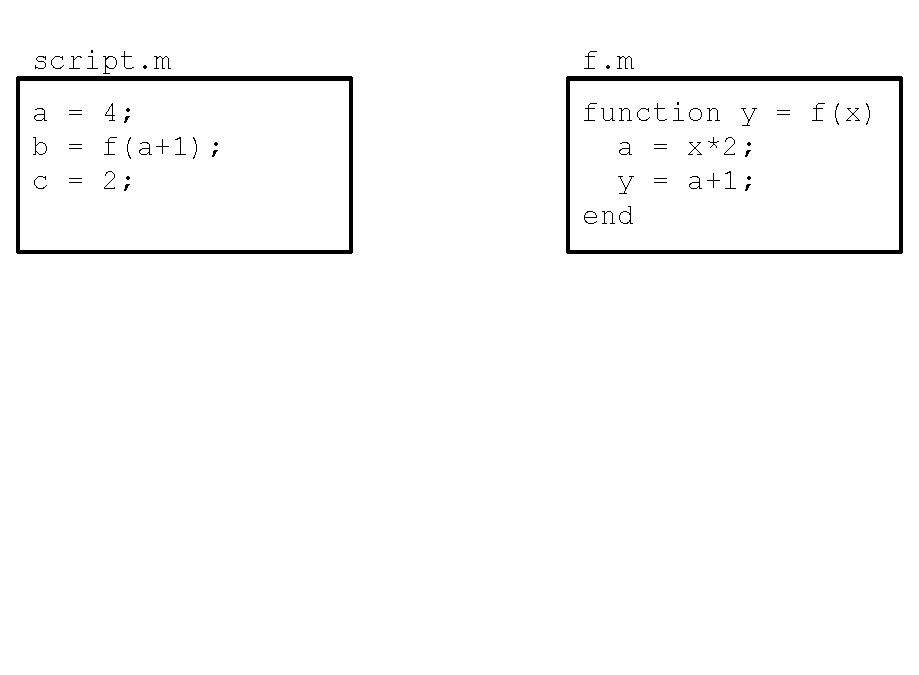
\includegraphics[width=\textwidth]{Pics/framkvaemd-falls-0}
\end{frame}
\begin{frame}{Framkvæmd}
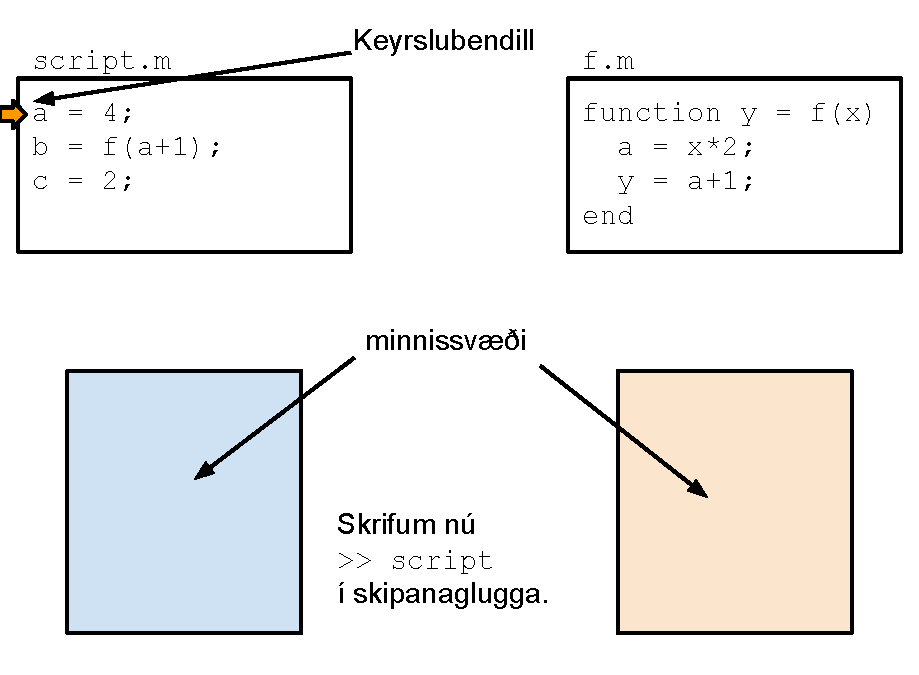
\includegraphics[width=\textwidth]{Pics/framkvaemd-falls-1}
\end{frame}
\begin{frame}{Framkvæmd}
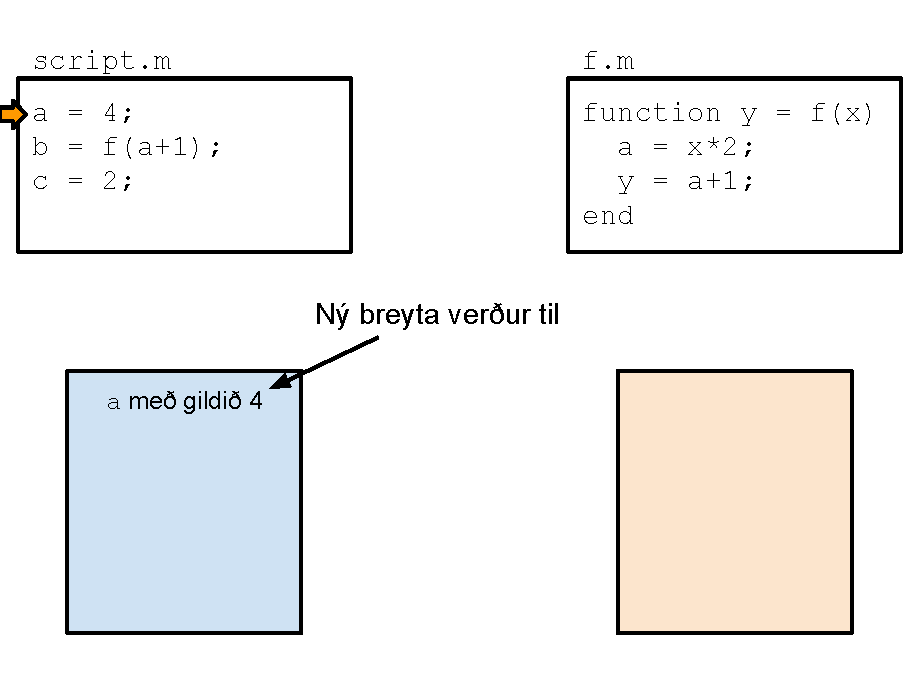
\includegraphics[width=\textwidth]{Pics/framkvaemd-falls-2}
\end{frame}
\begin{frame}{Framkvæmd}
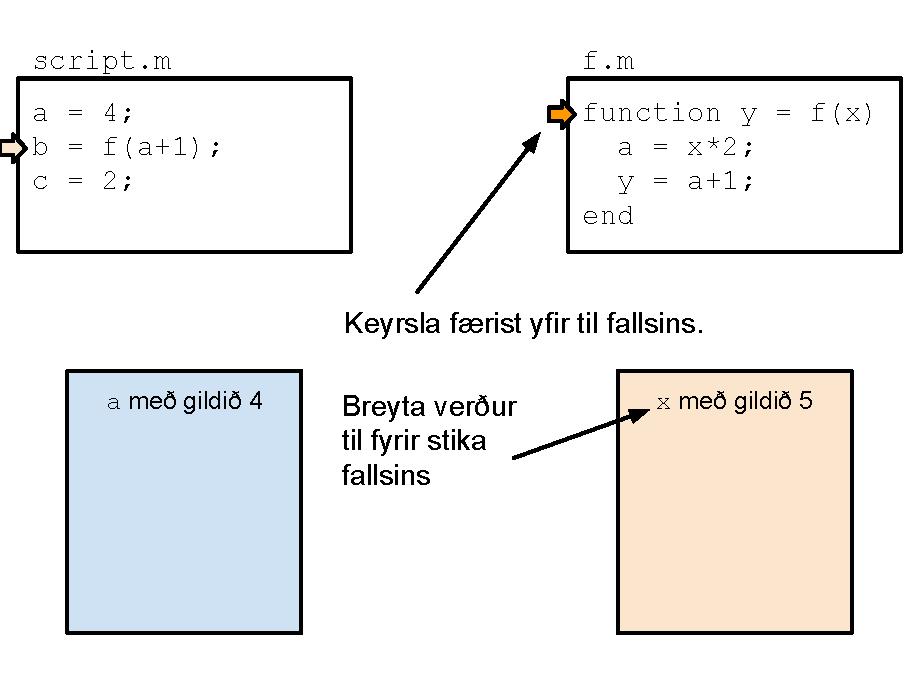
\includegraphics[width=\textwidth]{Pics/framkvaemd-falls-3}
\end{frame}
\begin{frame}{Framkvæmd}
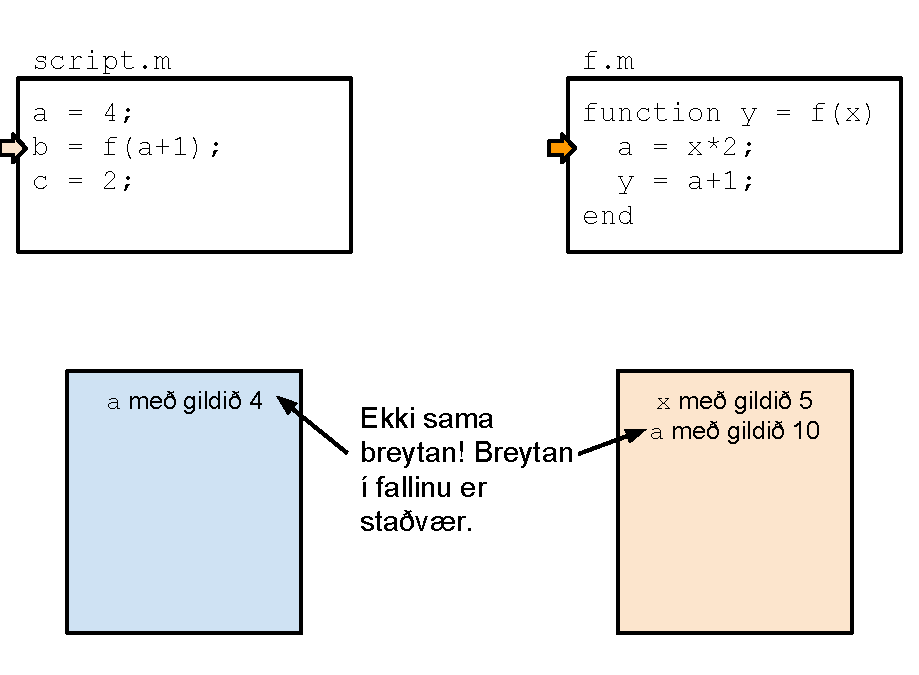
\includegraphics[width=\textwidth]{Pics/framkvaemd-falls-4}
\end{frame}
\begin{frame}{Framkvæmd}
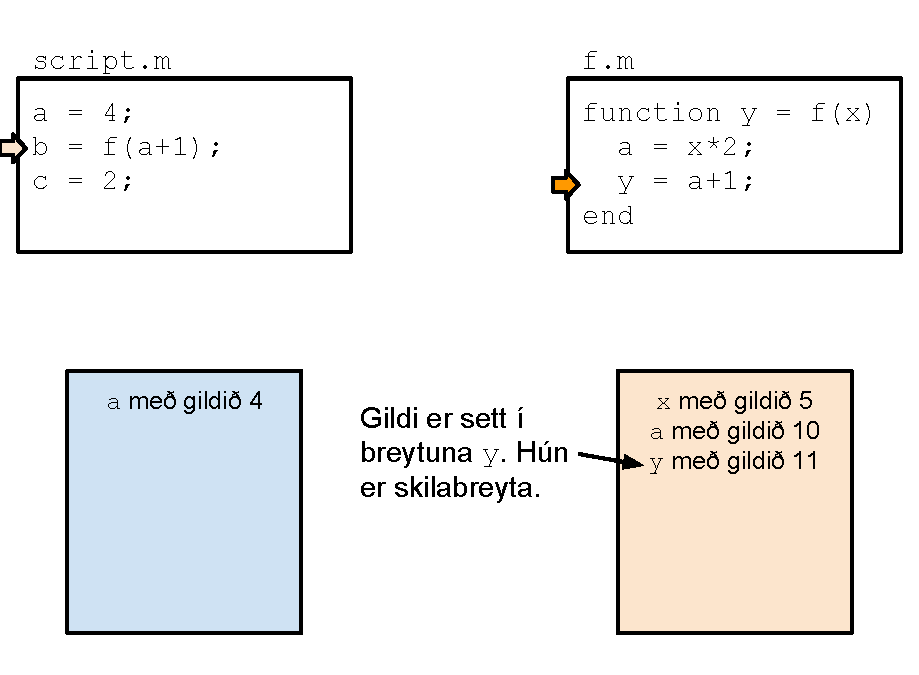
\includegraphics[width=\textwidth]{Pics/framkvaemd-falls-5}
\end{frame}
\begin{frame}{Framkvæmd}
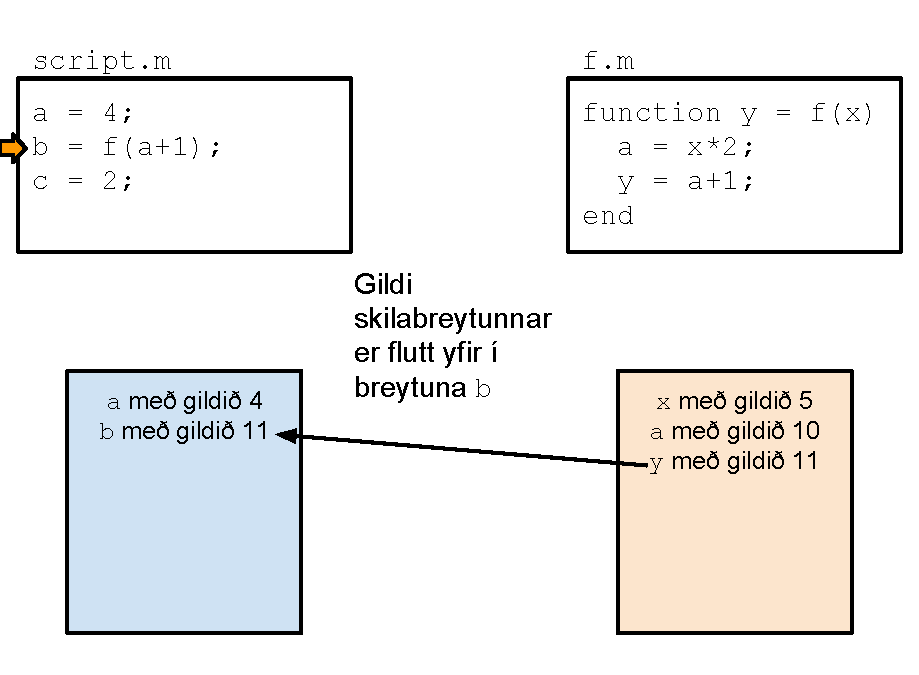
\includegraphics[width=\textwidth]{Pics/framkvaemd-falls-6}
\end{frame}
\begin{frame}{Framkvæmd}
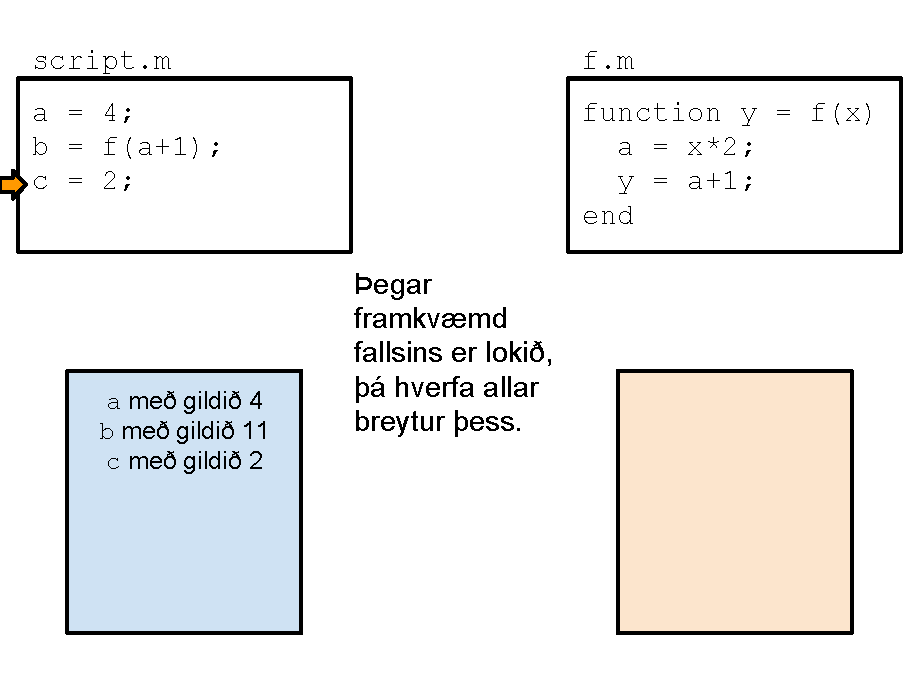
\includegraphics[width=\textwidth]{Pics/framkvaemd-falls-7}
\end{frame}

\begin{frame}{Fyrirlestraræfing}
\begin{enumerate}
 \item Skrifið fallið \texttt{celcToFahr}, sem breytir Celsíus hitastigi yfir í Fahrenheit ($f = c\cdot1.8 + 32$)
 \item Skilgreinið breytuna $z$ í skipanaglugganum. Skilgreinið líka fallið $fz$. Getur notendaskilgreinda fallið $fz$ notað breytuna z úr skipanaglugganum? Getur skipanaskrá gert það?
\end{enumerate}
\end{frame}

\section{Stýrisetningar}

\subsection{if (4.1)}

\begin{frame}{Stýrisetningin if}
\begin{columns}
\column{0.5\textwidth}
\begin{itemize}
 \item Hingað til hefur því verið haldið fram að hver einasta lína í falli eða skipanaskrá sé keyrð á eftir þeirri sem er fyrir ofan \pause
 \begin{itemize}
  \item \ldots það er lygi. \pause
 \end{itemize}
 \item Skipun til að velja hvort að ``blokk'' af kóða sé keyrð eða ekki er \texttt{if}
\end{itemize}
\column{0.5\textwidth}
\begin{center}
 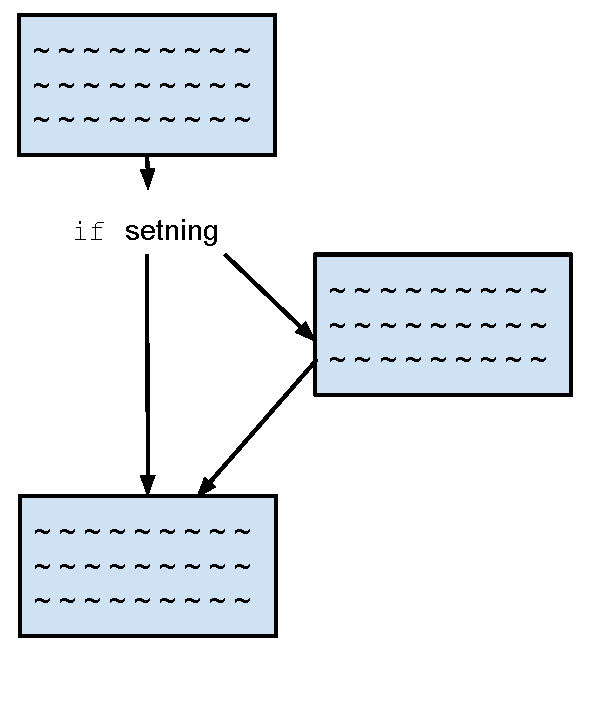
\includegraphics[width=0.8\linewidth]{Pics/if}
\end{center}
\end{columns}
\end{frame}

\begin{frame}[fragile]{Uppbygging if-skipunar}
\vspace{\baselineskip}
Hér eru skipanirnar einungis framkvæmdar ef ákveðið \emph{skilyrði} er uppfyllt.

\begin{verbatim}
if skilyrði
  skipun
  skipun
  ...
  skipun
end
\end{verbatim} 
Þetta skilyrði er \emph{rökyrðing} sem í einhverjum skilningi er sönn eða ósönn.

\end{frame}

\begin{frame}{Upprifjun - rökyrðingar}
\begin{itemize}
 \item Rökyrðingar (e. \emph{logical expressions}) vinna með \emph{sanngildi} í stað talna.
 \begin{itemize}
  \item Sanngildi eru tvö: \texttt{true} og ósatt \texttt{false}
  \item Í Matlab er oft notað $1$ og $0$ í stað \texttt{true} og \texttt{false}
 \end{itemize}
 \item Notum samanburðarvirkja (e. \emph{relational operators}) og rökvirkja (e. \emph{logical operators})
\end{itemize}
\end{frame}

\begin{frame}{Upprifjun - samanburðarvirkjar}
\begin{columns}
\column{0.5\textwidth}
\begin{itemize}
 \item Samanburðarvirkjar bera saman gildi og skila sanngildi (e. \emph{truth value}).
 \item Sanngildi hafa sitt eigið tag, \texttt{logical}
\end{itemize}
\column{0.5\textwidth}

\vspace{0.5cm}
Samanburðarvirkjar í Matlab: 

\vspace{0.2cm}
\begin{tabular}{ll}
\toprule
Virki&Merking\\
\midrule
\texttt{>}&stærri en\\
\texttt{<}&minni en\\
\texttt{>=}&stærri en eða jafn ($\geq$)\\
\texttt{<=}&minni en eða jafn ($\leq$)\\
\texttt{==}&jafnt og\\
\texttt{\~}\texttt{=}&ekki jafnt og\\
\bottomrule
\end{tabular}
\end{columns}
\end{frame}

\begin{frame}{Upprifjun - rökvirkjar}
Rökvirkjar vinna með sanngildi:
\begin{center}
\begin{tabular}{ll}
\toprule
Virki&Merking\\
\midrule
||& eða, skilar satt ef annað viðfangið er satt\\
\&\& & og, skilar satt ef bæði viðföngin eru sönn\\
\~{} &ekki, skilar öfugu við viðfangið\\
\bottomrule
\end{tabular}
\end{center}
Einnig er til rökfallið \texttt{xor}. Það tekur tvö viðföng og skilar ``annaðhvort eða''. Satt ef annað viðfangið er satt, en ekki ef bæði eru sönn.
\end{frame}

\begin{frame}[fragile]{Dæmi um if-setningar}
Inndregnu skipanirnar eru einungis keyrðar sé ákveðið skilyrði uppfyllt.
\begin{minted}[frame=lines]{matlab}
if x >= 0
    fprintf('Kvaðratrót %f er %f\n', x, sqrt(x));
end
\end{minted}

\begin{minted}[frame=lines]{matlab}
if q ~= 0
    fx = (4*d + h)/q;
end
\end{minted}

\end{frame}

\begin{frame}[fragile]{Stærra dæmi}
Þetta mætti setja í skipanaskrá og keyra:
\begin{minted}[frame=lines]{matlab}
% Biðja notanda um tölu og prenta út kvaðratrót hennar
num = input('Sláið inn tölu: ');

% Ef talan er neikvæð, þá breyta henni
if num < 0
    num = 0;
end
fprintf('Kvaðratrót %.1f er %.1f\n', num, sqrt(num));
\end{minted}
\end{frame}

\begin{frame}[fragile]{Skilyrði í if-setningu}
Athugið að Matlab reynir að túlka hvað svosem sett er í skilyrðishluta \texttt{if}-setningar sem rökgildi.

\begin{minted}[frame=lines]{matlab}
>> if -4
disp('Já, þetta er satt')
end
Já, þetta er satt
\end{minted}
Ath: Slæm hugmynd að notfæra sér þetta viljandi.
\end{frame}

\begin{frame}{Algeng villa}
\begin{itemize}
 \item Gerum ráð fyrir að notandi hafi verið að segja okkur hvort forrit eigi að halda áfram
 \begin{itemize}
  \item \texttt{svar = input('Halda áfram (J/N): ','s');}
 \end{itemize}
 \item Vitum ekki hvort notandinn sagði \texttt{'j'} eða \texttt{'J'}, svo við athugum hvort tveggja
 \begin{itemize}
  \item \texttt{if svar == 'J' || 'j'}
  \item Hvað er að þessu? \pause
 \end{itemize}
 \item Bókstafirnir eru túlkaðir sem tölur (sem eru ekki núll), svo þetta verður alltaf satt!
 \item Rétt útgáfa: \texttt{if svar == 'J' || svar == 'j'}
\end{itemize}
\end{frame}

\subsection{if og else (4.2)}

\begin{frame}[fragile]{if-else setningin}
\begin{columns}
\column{0.5\textwidth}
Getum valið á milli tveggja hópa af setningum með \texttt{if-else} setningunni
\begin{verbatim}
if skilyrði
    setningar
else
    aðrar setningar
end
\end{verbatim}
Ef skilyrðið er satt þá er fyrri setningahópurinn framkvæmdur, annars seinni
\column{0.5\textwidth}
\begin{center}
 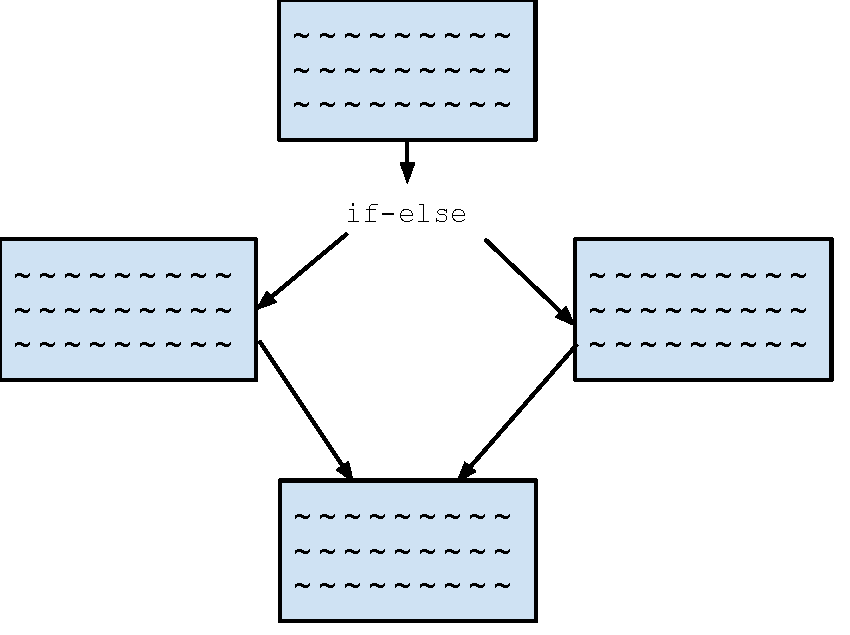
\includegraphics[width=\linewidth]{Pics/if-else}
\end{center}
\end{columns}
\end{frame}

\begin{frame}[fragile]{Dæmi um if-else setningar}
\begin{minted}[frame=lines]{matlab}
if rand() < 0.5
    disp('Þorskur');
else
    disp('Skjaldarmerki');
end
\end{minted}

\begin{minted}[frame=lines]{matlab}
rad = input('Sláðu inn radíus: ');
if rad < 0
    fprintf('%.2f er ólöglegur radíus\n', rad);
else
    area = pi * rad*rad;
    fprintf('Flatarmálið er %.2f\n', area);
end
\end{minted}
\end{frame}

\begin{frame}{fyrirlestrarræfing}
\begin{enumerate}
\setcounter{enumi}{2}
 \item Skrifið \texttt{if}-setningu sem prentar út villuskilaboð ef breytan \texttt{x} er minni en 0
 \item Skrifið \texttt{if}-setningu sem skrifar út hvort nemandi hafi fallið í námskeiði eða ekki (tvö mismunandi skilaboð).  Nemandi fellur ef prófeinkunn (\texttt{profeinkunn}) er lægri en 5.0
\end{enumerate}

\end{frame}

\subsection{Hreiðraðar if-setningar (4.3)}

\begin{frame}[fragile]{Upprifjun og lausn á fyrirlestraræfingu}
\texttt{if} skipun er notuð eigi að keyra ``blokk'' af skipunum þá og því aðeins að ákveðið \emph{skilyrði} hafi sanngildið ``satt''.
\begin{minted}[frame=lines]{matlab}
if x < 0 % Hér er skilyrðið ``x minna en 0''
    disp('Villa! x má ekki vera neikvæð.')
end
\end{minted}
\end{frame}

\begin{frame}[fragile]{Upprifjun og lausn á fyrirlestraræfingu}
\texttt{if} og \texttt{else} má nota saman til að velja á milli tveggja blokka.
\begin{minted}[frame=lines]{matlab}
if grade >= 5
    disp('Nemandinn nær prófinu!')
else
    disp('Nemandinn fellur á prófinu.')
end
\end{minted}
\end{frame}

\begin{frame}{Flóknari skilyrði}
\begin{itemize}
 \item Hvað ef möguleikarnir eru fleiri? \pause
 \begin{itemize}
  \item Nota margar \texttt{if}-setningar
  \item Nota hreiðraðar (e. \emph{nested}) \texttt{if}-setningar
  \item Nota \texttt{elseif}
  \item Nota \texttt{switch}-setningu
 \end{itemize}
\end{itemize}
\end{frame}

\begin{frame}{Dæmi: ``Gaffalfall''}
\begin{columns}
\column{0.5\textwidth}
Skoðum fallið $f(x)$:
\[
 f(x) =  \left \{
\begin{array}{ll}
1&, x < -1\\
x^2&, -1 \leq x \leq 2\\
4&, x > 2
\end{array}
\right.
\]
Hvernig getum við skrifað það í Matlab?
\column{0.5\textwidth}
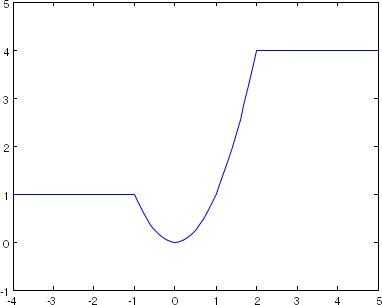
\includegraphics[width=\linewidth]{Pics/forked-function}
\end{columns}
\end{frame}

\begin{frame}[fragile]{Möguleiki: Þrjár if-setningar}
\begin{columns}
\column{0.5\textwidth}
\begin{minted}[frame=lines]{matlab}
if x < -1
    y = 1;
end

if x >= -1 && x <= 2
    y = x^2;
end

if x > 2
    y = 4;
end
\end{minted}
\column{0.5\textwidth}
\begin{itemize}
 \item Virkar, en ekki mjög sniðugt
 \item Ef fyrsta skilyrðið er satt, þá eru hvorug hinna sönn, en þau eru samt reiknuð
 \begin{itemize}
  \item Ekki hagkvæmt
 \end{itemize}
 \item Kóðinn gefur til kynna að öll skilyrðin séu óháð, en þau eru það ekki
\end{itemize}
\end{columns}
\end{frame}

\begin{frame}[fragile]{Möguleiki: Hreiðraðar if-setningar}
\begin{columns}
\column{0.5\textwidth}
\begin{minted}[frame=lines]{matlab}
if x < -1
    y = 1;
else
    if x <= 2
        y = x^2;
    else
        y = 4;
    end
end
\end{minted}
\column{0.5\textwidth}
\begin{itemize}
 \item Notum nýtt trix - \texttt{if} setning inni í \texttt{if} setningu
 \item Vitum að ef $x$ er ekki minna en -1, þá hlýtur það að vera einn af hinum tveimur möguleikunum
 \item Veljum á milli þeirra með seinni \texttt{if}-setningunni
 \item Galli (hér): Kóðinn lítur ekki lengur út eins og skilgreining fallsins
\end{itemize}
\end{columns}
\end{frame}

\begin{frame}[fragile]{Möguleiki: elseif}
\begin{columns}
\column{0.5\textwidth}
\begin{minted}[frame=lines]{matlab}
if x < -1
    y = 1;
elseif x>=-1 && x<=2
    y = x^2;
elseif x > 2
    y = 4;
end
\end{minted}
\column{0.5\textwidth}
\begin{itemize}
 \item Mjög svipað og hreiðraðar if-setningar
 \begin{itemize}
  \item Þetta er er þó læsilegra, sérstaklega ef möguleikarnir eru margir
  \item Hér hefur elseif líka þann kost að líkjast upphaflegri lýsingu á vandamálinu (fallinu)
 \end{itemize}
 \item Möguleikarnir eru metnir hver á fætur öðrum
\end{itemize}
Getum við gert betur?
\end{columns}
\end{frame}

\begin{frame}[fragile]{Möguleiki: elseif}
\begin{columns}
\column{0.5\textwidth}
\begin{minted}[frame=lines]{matlab}
if x < -1
    y = 1;
elseif x <= 2
    y = x^2;
else
    y = 4;
end
\end{minted}
\column{0.5\textwidth}
\begin{itemize}
 \item Óþörf skilyrði hafa hér verið fjarlægð
 \item Niðurstaða er alltaf sú sama, vegna röð samanburðanna
 \item Örlítið skilvirkara, ekki jafn líkt upphaflega vandamálinu
 \begin{itemize}
  \item Er það betra?
 \end{itemize}
\end{itemize}
\end{columns}
\end{frame}

\begin{frame}[fragile]{Annað dæmi um elseif}
\begin{columns}
\column{0.4\textwidth}
Breytt úr talnaeinkunn yfir í stafaeinkunn:
\column{0.6\textwidth}
\begin{minted}[frame=lines]{matlab}
if numGrade == 9 || numGrade == 10
    charGrade = 'A';
elseif numGrade == 8
    charGrade = 'B';
elseif numGrade == 7
    charGrade = 'C';
elseif numGrade == 6
    charGrade = 'D'
else
    charGrade = 'F';
end
\end{minted}
\end{columns}
\end{frame}

\subsection{Switch (4.4)}
\begin{frame}[fragile]{Annar möguleiki: switch}
\begin{columns}
\column{0.4\textwidth}
\begin{itemize}
 \item Oft er hægt að nota \texttt{switch} setningu í stað \texttt{if} setningar með marga \texttt{elseif} hluta
 \begin{itemize}
  \item Þegar mörg tilfelli hafa sömu útkomu má nota slaufusviga til að afmarka
  \item Undir lok \texttt{switch} getur komið \texttt{otherwise} (ekki \texttt{else})
 \end{itemize}

\end{itemize}

\column{0.6\textwidth}
\vspace{\baselineskip}
\begin{minted}[frame=lines]{matlab}
switch numGrade
    case {10, 9}
        charGrade = 'A';
    case 8
        charGrade = 'B';
    case 7
        charGrade = 'C';
    case 6
        charGrade = 'D';
    otherwise
        charGrade = 'F';
end
\end{minted}
\end{columns}
\end{frame}

\section{is-föll (4.6)}

\begin{frame}{is-Föll í Matlab}
\begin{itemize}
 \item Mörg föll í Matlab til að athuga hvort einhver eiginleiki gildi
 \begin{itemize}
  \item Þau skila sanngildi (satt/ósatt)
  \item Langflest þeirra byrja á enska orðinu ``is''
  \item Notuð til að athuga ýmislegt, t.d.
  \begin{itemize}
   \item tegund breytu (heiltala, kommutala, bókstafur, \ldots)
   \item gerð breytu (tala, vigur, fylki)
  \end{itemize}
 \end{itemize}
\end{itemize}
\end{frame}

\begin{frame}[fragile]{Dæmi: isletter fallið}
\begin{columns}
\column{0.35\textwidth}
\begin{itemize}
 \item \texttt{isletter} skilar \emph{satt} ef inntakið er bókstafur
 \begin{itemize}
  \item Þ.e. ekki tölustafur, greinarmerki eða sértákn
  \item Ræður við íslenska stafi
  \item Skilar \emph{ósatt} sé inntak ekki af taginu char
 \end{itemize}
\end{itemize}
\column{0.65\textwidth}
\begin{minted}[frame=lines]{matlab}
symb = input('Sláðu inn staf: ','s');
if isletter(symb)
    disp('Þetta er bókstafur');
else
    disp('Þetta er ekki bókstafur');
end
\end{minted}
\end{columns}
\end{frame}

\begin{frame}[fragile]{Dæmi: isempty fallið}
\begin{columns}
\column{0.3\textwidth}
\begin{itemize}
 \item \texttt{isempty} skilar \emph{satt} sé breyta tóm
 \begin{itemize}
  \item \emph{Ósatt} innihaldi breytan gildi
 \end{itemize}
 \item breytan þarf þó að vera skilgreind
\end{itemize}
\column{0.7\textwidth}
\begin{minted}[frame=lines]{matlab}
>> format compact
>> v = [];
>> isempty(v)
ans =  1
>> v = [1, 2];
>> isempty(v)
ans = 0
>> clear
>> isempty(v)
??? Undefined function or variable 'v'.
\end{minted}
\end{columns}
\end{frame}

\begin{frame}[fragile]{Dæmi: exist fallið}
\begin{columns}
\column{0.5\textwidth}
\begin{itemize}
 \item Hægt að athuga hvort breyta, fall eða annað sé skilgreint með fallinu \texttt{exist}
 \item Tekur inn nafn í streng
 \begin{itemize}
  \item Skilar 0 sé nafnið ekki skilgreint
  \item Aðrar tölur eftir gerð fyrirbrigðisins sem nafnið vísar til
 \end{itemize}
\end{itemize}
\column{0.5\textwidth}
\begin{minted}[frame=lines]{matlab}
>> x = 1;
>> exist('x')
ans =  1
>> exist('sin')
ans =  5
>> exist('y')
ans = 0
\end{minted}
\end{columns}
\end{frame}

\begin{frame}{Fleiri is-föll}
\begin{center}
\begin{tabular}{ll}
\toprule
Fall&Spurning\\
\midrule
\texttt{isnumeric}&Er inntakið tala?\\
\texttt{isinteger}&Er inntakið af heiltölutagi?\\
\texttt{iscolumn}&Er inntakið dálkvigur?\\
\texttt{isrow}&Er inntakið línuvigur?\\
\texttt{issorted}&Er inntakið raðaður vigur?\\
\texttt{isvarname}&Er inntakið strengur með löglegu breytunafni?\\
\bottomrule
\end{tabular}
\end{center}
\end{frame}


\end{document}
